\chapter{Exercise 8}
The purpose of this exercise is to understand and implement shadow mapping. 
This includes a deep understanding of the different coordinate spaces in the 
pipeline as well as mapping between these coordinate spaces. 

\section{Part 1, 2 and 3}
Following the instructions I rendered a teapot to the shadowmap, using 1 for lit areas
and 0 otherwise. I also succeded in retrieving UV coordinates from shadow map in the
fragment shader. We can see some results in the figure \ref{fig:exercise_8_1}.
\begin{figure}[ht!]
	\begin{center}
		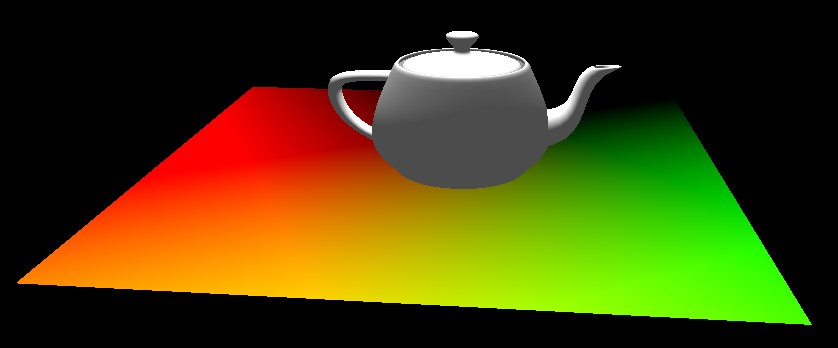
\includegraphics[width=1.0\textwidth]{figures/exercise_8_1}
	\end{center}
	\vspace{-4.5ex}\caption{Exercise 8 part 3 output}
	\label{fig:exercise_8_1} 
\end{figure}

\section{Part 4}
At last I used the shadow texture coordinates to lookup a color (1 or 0) in the shadow map texture.
Now with that knowledge I managed to darken the shadowed areas using mix function. 
\begin{figure}[ht!]
	\begin{center}
		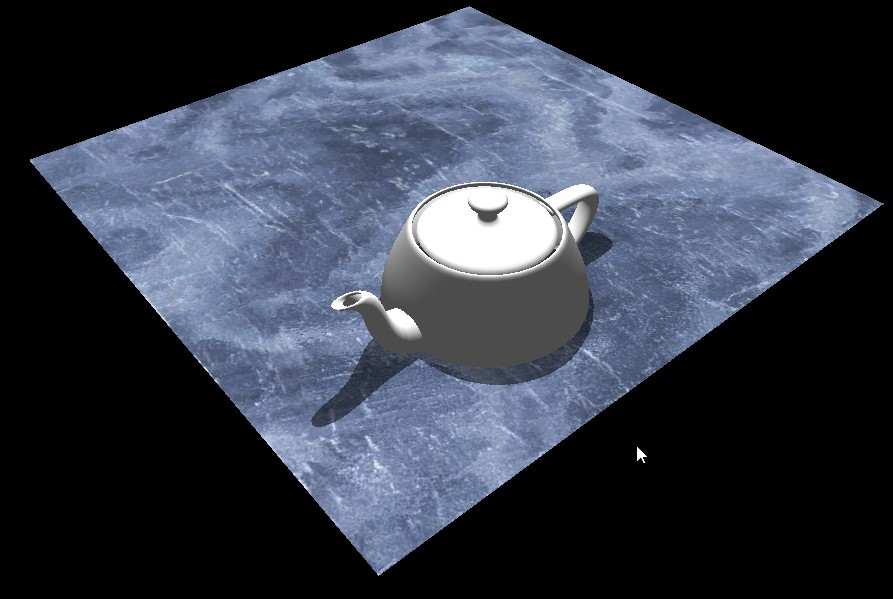
\includegraphics[width=1.0\textwidth]{figures/exercise_8_2}
	\end{center}
	\vspace{-4.5ex}\caption{Exercise 8 part 4 output}
	\label{fig:exercise_8_2} 
\end{figure} \\
A accomplished that using following code in the fragment shader:
\begin{lstlisting}[language=cpp, caption={Fragment shader - in main()}]
mat4 biasMatrix;
biasMatrix[0]=vec4(0.5, 0.0, 0.0, 0.0);
biasMatrix[1]=vec4(0.0, 0.5, 0.0, 0.0);
biasMatrix[2]=vec4(0.0, 0.0, 0.5, 0.0);
biasMatrix[3]=vec4(0.5, 0.5, 0.5, 1.0);
vec4 coordinates = biasMatrix * lightViewProjection * vWorldCoordinate;
vec2 shadowUV = (coordinates / coordinates.w).xy;
vec4 texColor = texture(texture1, vTextureCoordinate);
vec4 shadowColor = texture(shadowMap, shadowUV);
if(shadowColor.x == 1.0)
	fragColor = texColor;
else
	fragColor = mix(texColor, shadowColor, 0.5);
\end{lstlisting}